\chapter{Methodology}
\label{mt:methodology}

In this section, we will walk through all the organizational aspects related to the project: configuration management and \gls{cicd} workflows.

\section{Configuration Management}

Configuration management can be defined as a process that ensures the consistency and quality of a project/product through its life cycle and the various changes it undergoes. Sometimes the term is mistaken for version control, but in fact configuration management includes version control~\cite{hammond2012version}.

In this subsection we will talk about the different technologies and tools that have been used in order to keep a decent control of configuration management.

\subsection{Git \& GitHub}

As mentioned above, version control is a part of configuration management and is responsible for recognizing and managing the various changes of software code. Version control systems are software tools that help teams manage changes to source code over time. 

For this project Git has been the clear option since it is the market leader due to its huge speed and its branch and merge functionality, among others. Taken from its website \enquote{Git is a free and open source distributed version control system designed to handle everything from small to very large projects with speed and efficiency}.

GitHub is essentially a remote repository hosting platform for Git. It allows developers to work together on the same project from anywhere~\cite{chacon2014pro}.

\subsection{Git Workflow}

A Git workflow is a template for how to use git to accomplish work in a consistent and productive manner. Git is extremely flexible when it comes to managing changes, so there is no imposed or standardized process. When working with a team on a project, it is important to make sure that the entire team is familiar with how changes will be applied. 

Gitflow has been chosen for this project because of its versatility and the ability to generate branches for each of the features needed for the project, Figure~\ref{fig:gitflow-example}. In our case, it will be extremely useful to be able to develop each of the modules/micro-services of the system in parallel~\cite{driessen2010successful}.

\begin{figure}[H]
    \centering
    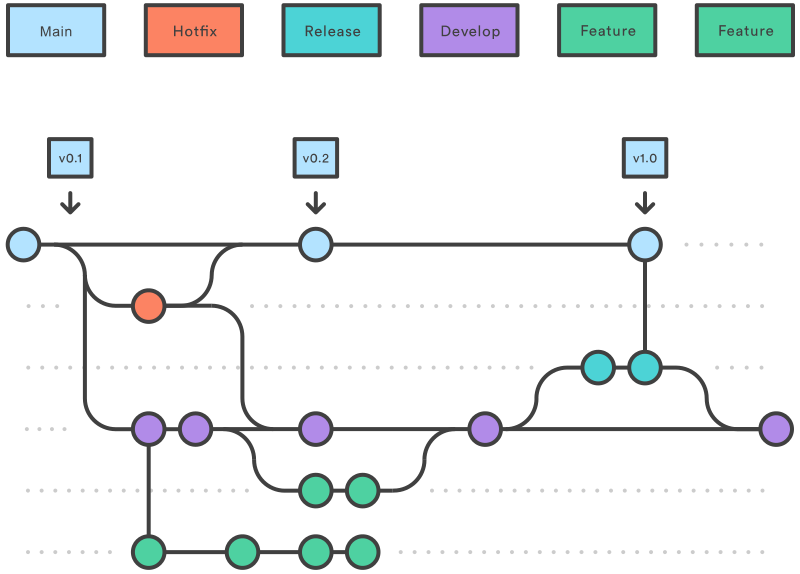
\includegraphics[width=0.55\textwidth]{figures/gitflow.png}
    \caption{Gitflow Scheme, Source: www.atlassian.com}
    \label{fig:gitflow-example}
\end{figure}

\section{CI/CD Workflows}

One of the main goals during the design phase of this thesis is to have a high level of automation to be able to maintain all the different development processes. Luckily GitHub provides us with a powerful tool for creating custom workflow pipelines, called GitHub actions. These workflows must be located in a folder called \textbf{.github/workflows}, in the root of the repository in different "YAML" files~\cite{github2020actions}.

GitHub actions fees depend on computing time and the runner's \gls{os}. Runners are responsible for executing the different jobs specified in a workflow, Tab~\ref{tab:action-fees} shows the different prices.

\begin{table}[h]
\centering
\caption{Runner Fees}
\label{tab:action-fees}
\begin{tabular}{@{}ll@{}}
\toprule
Linux             & \$0.008/min \\ \midrule
Windows           & \$0.016/min \\ \midrule
macOs             & \$0.08/min  \\ \midrule
Self-hosted       & Free        \\ \midrule
Public repository & Free       
\end{tabular}
\end{table}

\newpage
\subsection{Self-hosted Runner}

\begin{lstlisting}[language=bash, caption=Set up Self-hosted Runner,label={lst:self-hosted-runner}]
$ curl -o actions-runner-linux-x64-2.287.1.tar.gz -L https://github.com/actions/runner/releases/download/v2.287.1/actions-runner-linux-x64-2.287.1.tar.gz
$ tar xzf ./actions-runner-linux-x64-2.287.1.tar.gz
$ ./config.sh --url https://github.com/username/repository --token "YOUR TOKEN"
$ ./run.sh
$ sudo ./svc.sh install #this will create a systemd daemon to start the runner on start up
\end{lstlisting}

Self-hosted runners offer more control of hardware, \gls{os}, and software tools than GitHub-hosted runners provide. With self-hosted runners, you can choose to create a custom hardware configuration with more processing power or memory to run larger jobs, install software available on your local network, and choose an \gls{os} not offered by GitHub-hosted runners. Self-hosted runners can be physical, virtual, in a container, on-premises, or in a cloud.

To add a self-hosted runner, is as simple as going to the actions section in the repository settings and follow the instructions, Listing~\ref{lst:self-hosted-runner} shows the steps used to configure a Linux based runner for the project. From now on, our self-hosted runner will listen for jobs from our GitHub repository and start executing them whenever a workflow is triggered.

\subsection{Workflow Definition}

Two of the most important aspects to take into consideration when defining a workflow, are the branches or events that will trigger it and the jobs and tasks to be executed. Note that these jobs do not necessarily have to be sequentially executed, in fact they run in parallel by default. Nonetheless, GitHub actions allows us to establish dependencies between jobs, so that certain ones are executed before others.

Triggering events must be defined under the \enquote{on}: tag. Listing~\ref{lst:trigger-options} shows an example of a couple of interesting ones, for more information about triggering events follow the instructions in the action's documentation.

\begin{lstlisting}[caption=Common Workflow Triggers,label={lst:trigger-options}]
on:
  push:
    branches: [only when specific branches are pushed]
    branches-ignore: [ignored branches]
    paths: # triggers when a push to specific files occurs
        - '**.go'
  pull_request:
    types: [pull request activity type]
  workflow_dispatch: # allows the workflow to be triggered manually
\end{lstlisting}

As for the job definition, they all must be declared under the \enquote{job} tag. Jobs run in parallel by default as we explained before. To run them sequentially, you can define dependencies as Listing~\ref{lst:jobs-definition} shows. Also, the runner which will execute the job, needs to be chosen in the definition.

\begin{lstlisting}[caption=Job Dependencies Definition,label={lst:jobs-definition}]
jobs:
  jobA:
    runs-on: [self-hosted] # the job will be forwarded to our self-hosted runner
  jobB:
    runs-on: [ubuntu-latest] # the job will be executed in a hosted ubuntu machine
    needs: jobA
  jobC:
    runs-on: [self-hosted]
    if: ${{ always() }} #jobC will execute regardless of jobA & jobB output
    needs: [jobA, jobB]
\end{lstlisting}

The most powerful feature about GitHub actions is the integration with its whole ecosystem. So for instance, each job has a list of steps which are always executed sequentially and they all need to pass, in order for the job to successfully finish. These task can be either manually specified or reused from the Action's marketplace, where everyone can either upload or reuse published actions. To use any of them, is as simple as specifying the dependency \enquote{publisher/actions@version}. Listing~\ref{lst:step-definition} shows an example of a reused action from the marketplace.

Another useful feature is the \enquote{secrets} environment, which lets you define repository level environment variables that need to be off the code, i.e, \gls{api} keys, tokens or cryptography private keys.

\begin{lstlisting}[caption=Steps Definition,label={lst:step-definition}]
steps:
- uses: actions/first-interaction@v1 # dependency definition
  with:
    repo-token: ${{ secrets.GITHUB_TOKEN }} # GitHub environment variable
    issue-message: 'message that will be displayed on users' first issue'
    pr-message: 'message that will be displayed on users' first pr'
\end{lstlisting}

\section{Application to Our Use Case}
\label{sec:application-use-case}

This section delineates how the methodologies discussed in this chapter are applied to our specific use case, which involves the development and deployment of blockchain nodes on \gls{aws}, managed and automated through GitHub actions. The aim is to elucidate the practical application of configuration management and \gls{cicd} workflows in the context of a blockchain-based project, ensuring a seamless and efficient development lifecycle.

\subsection{Architecture Overview}

The architecture of our project is designed to optimize performance, security, and scalability. The blockchain nodes, the backbone of our application, are hosted on \gls{aws}, providing robust and scalable cloud infrastructure. The codebase for the project resides on GitHub, which acts as the central repository for version control and collaboration among the development team.

To visualize the integration and interaction between different components of our project, an architecture diagram is essential. Figure~\ref{fig:architecture-diagram} illustrates the overall architecture, focusing on high availability and high scalability of the service thanks to the \gls{alb} which supports the \gls{grpc} protocol natively.

\begin{figure}[H]
    \centering
    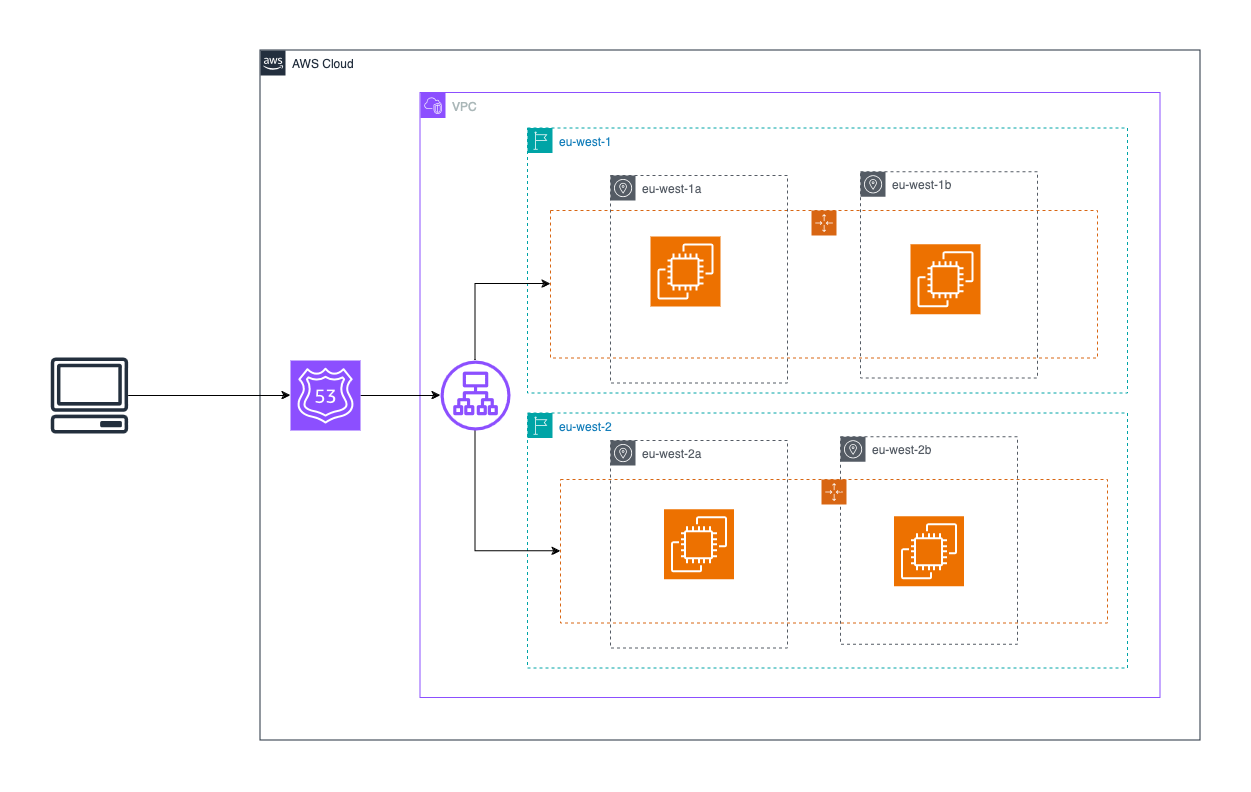
\includegraphics[width=\textwidth]{figures/aws.png}
    \caption{Overall Architecture Diagram}
    \label{fig:architecture-diagram}
\end{figure}

\newpage
\subsection{Deployment Sequence}
The deployment workflow is a critical aspect of our project, ensuring that the latest codebase changes are automatically tested, built, and deployed to the AWS environment. This process is facilitated by GitHub Actions, which automates the workflow based on specific triggers, such as a push to the main branch or a pull request.

A detailed diagram of the deployment workflow helps in understanding the sequence of events from code commit to deployment. Figure~\ref{fig:deployment-workflow-diagram} depicts this workflow, including the steps taken by GitHub Actions to deploy the application onto \gls{aws}.

\begin{figure}[H]
    \centering
    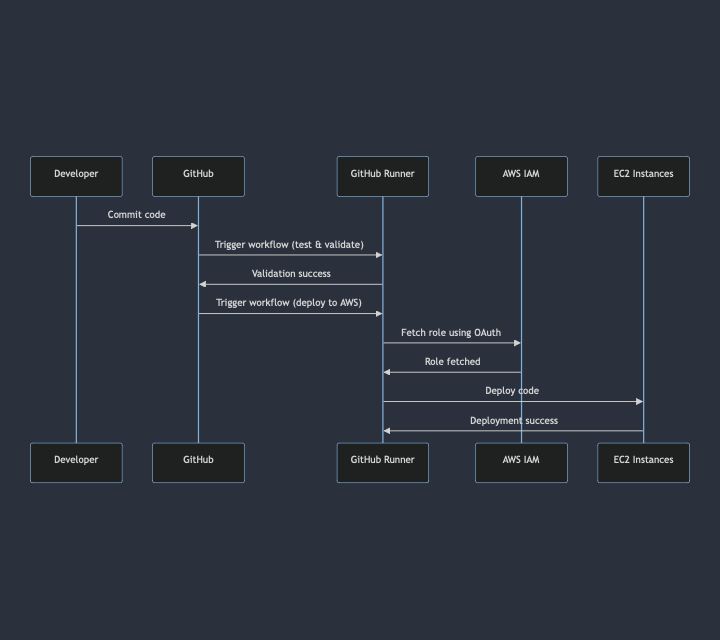
\includegraphics[width=\textwidth]{figures/sequence.png}
    \caption{Deployment Workflow Diagram}
    \label{fig:deployment-workflow-diagram}
\end{figure}

\subsection{Implementation Details}
The implementation of our use case begins with committing code changes to the GitHub repository. These changes trigger predefined GitHub Actions workflows.

The workflows include various jobs, such as linting, testing, building, and deploying. Each job is executed in an environment specified by the workflow, with most deployment tasks directed to self-hosted runners equipped to interact with \gls{aws} services. These runners use the OAuth protocol to authenticate against \gls{iam} in \gls{aws}, ensuring that the deployment process is both secure and efficient.

Upon successful completion of the deployment job, the updated application is live, ready to be accessed by users. This automated workflow not only minimizes human error but also significantly accelerates the development lifecycle, allowing for rapid iteration and feedback.

In conclusion, the application of configuration management and \gls{cicd} workflows to our use case exemplifies a modern, efficient, and scalable approach to software development and deployment. By leveraging industry-standard tools and practices, we ensure that our blockchain project remains at the forefront of technological advancements.
